\subsection{连续同态与严格态射}

命题 23 同态 \(f\)（拓扑群 \(\mathbf{G}\) 到拓扑群 \(\mathbf{G}'\) 中的）在 \(\mathbf{G}\) 上连续，当且仅当它在 \(\mathbf{G}\) 的一点处连续。

设 \(f\) 在一点 \(a \in \mathbf{G}\) 处连续；则若 \(\mathbf{V}'\) 是 \(f(a)\) 的任一邻域，\(\mathbf{V} = f^{-1}(\mathbf{V}')\) 是 \(a\) 的一个邻域。因而若 \(x\) 是 \(\mathbf{G}\) 的任一点，我们有

\[
f (x a ^ {- 1} \mathrm{V}) = f (x) [ f (a) ] ^ {- 1} f (\mathrm{V}) \subset f (x) [ f (a) ] ^ {- 1} \mathrm{V} ^ {\prime},
\]

因而 \(f\) 在 \(x\) 处连续。

拓扑群 G 到拓扑群 \(G'\) 中的连续同态也称为 G 到 \(G'\) 中的（对拓扑群结构而言的）态射。

设 \(f\) 是拓扑群 \(G\) 到拓扑群 \(G'\) 中的一个连续同态；原像 \(H = f^{-1}(e')\)——这里 \(e'\) 是 \(G'\) 的单位元——是 \(G\) 的一个正规子群，且 \(f(G)\) 是 \(G'\) 的一个子群。考虑典范分解 \(f = \psi \circ \overline{f} \circ \varphi\)，其中 \(\varphi\) 是典范映射 \(G \to G/H\)，\(\psi\) 是典范单射 \(f(G) \to G'\)，最后 \(\overline{f}\) 是商群 \(G/H\) 到子群 \(f(G)\) 上的一个连续双射同态（第一章 § 3 第 5 目）；称 \(\overline{f}\) 为伴随于 \(f\) 的双射同态。一般地说，\(f\) 不是拓扑群的一个同构。

例如，设 \(G'\) 是一个非离散拓扑群，G 是把离散拓扑赋予 \(G'\) 所得的拓扑群；则 G 到 \(G'\) 中的恒等映射是连续双射同态，但不是双连续的。

定义 1 拓扑群 G 到拓扑群 \(\mathbf{G}'\) 中的连续同态称为 G 到 \(\mathbf{G}'\) 中的严格态射，如果双射同态 \(\overline{f}\)（从 \(\mathbf{G}/f^{-1}(e')\) 到 \(f(\mathbf{G})\) 上的，伴随于 \(f\)）是拓扑群的一个同构（换言之，如果 \(\overline{f}\) 是双连续的）。

因此拓扑群 G 到拓扑群 \(G'\) 上的一个同构是 G 到 \(G'\) 上的一个双射严格态射。

命题 24 设 \(f\) 是拓扑群 \(G\) 到拓扑群 \(G'\) 中的一个连续同态。则下列三个命题等价：a) \(f\) 是严格态射。

\begin{enumerate}
\def\labelenumi{\alph{enumi})}
\setcounter{enumi}{1}
\item
  在 \(f\) 下，\(\mathbf{G}\) 中每个开集的像是 \(f(\mathbf{G})\) 中的一个开集。
\item
  在 \(f\) 下，\(G\) 的单位元的每个邻域的像是 \(G'\) 的单位元的一个邻域。
\end{enumerate}

鉴于第 4 目引理 2，a) 与 b) 的等价性由定义立即得出（第一章 § 5 第 3 目命题 5）。b) 与 c) 的等价性是第 5 目命题 15 的一个特殊情形，只要注意到 G 连续作用在 \(f(\mathbf{G})\) 上，其外法则是 \((s, f(t)) \to f(st)\)。

注。1) 由命题 24 的条件 b) 可得，拓扑群到离散群中的每个连续同态都是严格态射。

若 G 是紧的且 \(f(\mathbf{G})\) 是 Hausdorff 的，则伴随于 f 的双射同态 \(\overline{f}\) 是双连续的（第一章 § 10 第 2 目定理 1 推论 2，以及第 1 目命题 5 推论 4）。因此紧群到 Hausdorff 群中的每个连续同态都是严格态射。

\pandocbounded{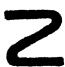
\includegraphics[keepaspectratio]{images/part002_802da4a7.jpg}}

\begin{enumerate}
\def\labelenumi{\arabic{enumi})}
\setcounter{enumi}{1}
\item
  设 \(f\) 是 \(G\) 到 \(G'\) 中的一个严格态射，\(g\) 是 \(G'\) 到 \(G''\) 中的一个严格态射。若 \(f\) 是满射或 \(g\) 是单射，则由命题 24 立即得出 \(g \circ f\) 是 \(G\) 到 \(G''\) 中的一个严格态射。但如果前面两个条件没有一个满足，这个结论就未必成立，即使 \(f\) 是单射且 \(g\) 是满射（习题 19）。
\item
  设 \(f\) 是拓扑群 \(G\) 到拓扑群 \(G'\) 中的一个连续同态，\(H\) 是 \(G\) 的一个正规子群。\(f\) 诱导一个同态 \(g\)（群 \(G / H\) 到商群 \(f(G) / f(H)\) 上的）。这个同态 \(g\) 是连续的。此外，若 \(f\) 是 \(G\) 到 \(G'\) 中的一个严格态射，则 \(g\) 是 \(G / H\) 到 \(f(G) / f(H)\) 上的一个严格态射；因为若 \(U\) 在 \(G / H\) 中是开的，且以 \(\varphi\)（相应地 \(\varphi'\)）表示 \(G\) 到 \(G / H\) 上{[}相应地 \(f(G)\) 到 \(f(G) / f(H)\) 上{]}的典范映射，则有 \(g(u) = \varphi'(f(\varphi^{-1}(u)))\)，而由于 \(\varphi^{-1}(u)\) 在 \(G\) 中是开的，可知 \(g(u)\) 在 \(f(G) / f(H)\) 中是开的，这就证明了我们的断言。
\end{enumerate}

